\documentclass[../main]{subfiles}
\usetikzlibrary{arrows.meta,calc,patterns,decorations.pathmorphing}

\begin{document}

\chapter{Principios fundamentales de la mecánica de fluidos}

\section{Bernoulli, Torricelli, Venturi y Pitot}

La mecánica de fluidos es una rama de la física que estudia el comportamiento de los líquidos y gases en reposo y en movimiento. Cuatro conceptos fundamentales en este campo son los principios de Bernoulli, Torricelli, Venturi y Pitot. Estos principios están interrelacionados y tienen numerosas aplicaciones en la ingeniería y la vida cotidiana.

\subsection{Principio de Bernoulli}

El principio de Bernoulli, formulado por Daniel Bernoulli en el siglo XVIII, es uno de los pilares de la mecánica de fluidos.

\info{Principio de Bernoulli}{
El principio de Bernoulli establece que en un fluido ideal\footnote{Un fluido hipotético sin viscosidad ni fricción interna} en régimen estacionario, la energía total en un punto de una línea de corriente es constante. Se expresa matemáticamente como:

\begin{equation}
P + \frac{1}{2}\rho v^2 + \rho g h = \text{constante}
\end{equation}

Donde:
\begin{itemize}
    \item $P$: Presión del fluido [Pa]
    \item $\rho$: Densidad del fluido [kg/m³]
    \item $v$: Velocidad del fluido [m/s]
    \item $g$: Aceleración debida a la gravedad [m/s²]
    \item $h$: Altura respecto a un nivel de referencia [m]
\end{itemize}
}

Esta ecuación relaciona la presión, la velocidad y la altura de un fluido en movimiento. Una consecuencia importante del principio de Bernoulli es que, al aumentar la velocidad de un fluido, su presión disminuye, y viceversa.

\ejemplo{Ejemplo del Principio de Bernoulli}{
Consideremos un tubo horizontal con un estrechamiento. Si el diámetro en la sección ancha es 10 cm y en la estrecha es 5 cm, y la velocidad en la sección ancha es 2 m/s, podemos calcular la velocidad en la sección estrecha usando la ecuación de continuidad:

\begin{equation}
A_1v_1 = A_2v_2
\end{equation}

Donde $A$ es el área de la sección transversal y $v$ la velocidad.

$\pi (0.05\text{ m})^2 v_2 = \pi (0.025\text{ m})^2 (2\text{ m/s})$

$v_2 = 8\text{ m/s}$

Según Bernoulli, la presión en la sección estrecha será menor que en la sección ancha debido a esta mayor velocidad.
}

\subsection{Teorema de Torricelli}

El teorema de Torricelli, desarrollado por Evangelista Torricelli en el siglo XVII, es una aplicación específica del principio de Bernoulli.

\info{Teorema de Torricelli}{
El teorema de Torricelli describe la velocidad de salida de un líquido a través de un orificio en un recipiente. Se expresa como:

\begin{equation}
v = \sqrt{2gh}
\end{equation}

Donde:
\begin{itemize}
    \item $v$: Velocidad de salida del líquido [m/s]
    \item $g$: Aceleración debida a la gravedad [m/s²]
    \item $h$: Altura del líquido sobre el orificio [m]
\end{itemize}
}

Este teorema se deriva del principio de Bernoulli, considerando que la presión en la superficie del líquido y en el orificio es la misma (presión atmosférica) y que la velocidad en la superficie es despreciable.

\ejemplo{Ejemplo del Teorema de Torricelli}{
Supongamos un tanque de agua con un pequeño orificio en su base. Si la altura del agua sobre el orificio es de 4 metros, ¿cuál será la velocidad de salida del agua?

Aplicando la ecuación de Torricelli:

\begin{equation}
v = \sqrt{2 \times 9.8\text{ m/s}^2 \times 4\text{ m}} = 8.85\text{ m/s}
\end{equation}

Por lo tanto, el agua saldrá del orificio a una velocidad de aproximadamente 8.85 m/s.
}

\subsection{Efecto Venturi}

El efecto Venturi, descubierto por Giovanni Battista Venturi en el siglo XVIII, es otra aplicación del principio de Bernoulli.

\info{Efecto Venturi}{
El efecto Venturi se produce cuando un fluido en movimiento dentro de un conducto cerrado disminuye su presión al aumentar la velocidad después de pasar por una zona de sección menor. Se puede expresar matemáticamente usando la ecuación de Bernoulli:

\begin{equation}
P_1 + \frac{1}{2}\rho v_1^2 = P_2 + \frac{1}{2}\rho v_2^2
\end{equation}

Donde los subíndices 1 y 2 se refieren a las condiciones antes y en el estrechamiento, respectivamente.
}

El efecto Venturi tiene numerosas aplicaciones prácticas, como en carburadores, sistemas de riego y dispositivos de medición de flujo.

\ejemplo{Ejemplo del Efecto Venturi}{
Un tubo Venturi se utiliza para medir el flujo de agua en una tubería. Si la presión en la sección ancha es de 200 kPa y en la sección estrecha es de 150 kPa, y la velocidad en la sección ancha es de 2 m/s, podemos calcular la velocidad en la sección estrecha:

$200000\text{ Pa} + \frac{1}{2} \times 1000\text{ kg/m}^3 \times (2\text{ m/s})^2 = 150000\text{ Pa} + \frac{1}{2} \times 1000\text{ kg/m}^3 \times v_2^2$

Resolviendo para $v_2$:

$v_2 = \sqrt{2 \times \frac{200000 - 150000 + 1000 \times 2^2/2}{1000}} = 10\text{ m/s}$

La velocidad en la sección estrecha es de 10 m/s.
}

\subsection{Tubo de Pitot}

El tubo de Pitot, inventado por Henri Pitot en el siglo XVIII, es un instrumento que utiliza los principios de Bernoulli para medir la velocidad de un fluido.

\info{Tubo de Pitot}{
Un tubo de Pitot mide la diferencia entre la presión total (o de estancamiento) y la presión estática de un fluido en movimiento. La velocidad del fluido se puede calcular usando la ecuación:

\begin{equation}
v = \sqrt{\frac{2(P_t - P_s)}{\rho}}
\end{equation}

Donde:
\begin{itemize}
    \item $v$: Velocidad del fluido [m/s]
    \item $P_t$: Presión total [Pa]
    \item $P_s$: Presión estática [Pa]
    \item $\rho$: Densidad del fluido [kg/m³]
\end{itemize}
}

Los tubos de Pitot se utilizan comúnmente en aeronaves para medir la velocidad del aire y en sistemas de ventilación para medir el flujo de aire.

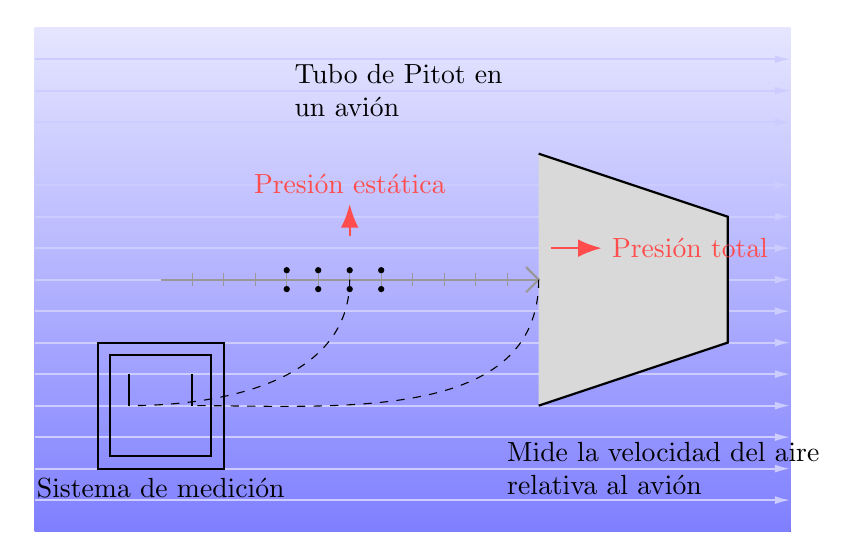
\begin{tikzpicture}[scale=0.8]
    % Definición de colores
    \colorlet{tubecolor}{gray!80}
    \colorlet{aircolor}{blue!20}
    \colorlet{pressurecolor}{red!70}

    % Fondo (cielo)
    \fill[top color=blue!10,bottom color=blue!50] (-6,-4) rectangle (6,4);

    % Flujo de aire
    \foreach \y in {-3.5,-3,...,3.5}
    {
        \draw[aircolor,thick,-{Latex[length=2mm,width=1mm]}] (-6,\y) -- (6,\y);
    }

    % Cuerpo principal del avión (simplificado)
    \fill[gray!30] (2,-2) -- (5,-1) -- (5,1) -- (2,2) -- cycle;
    \draw[thick] (2,-2) -- (5,-1) -- (5,1) -- (2,2);

    % Tubo de Pitot
    \draw[tubecolor,thick] (-4,0) -- (2,0);
    \draw[tubecolor,thick] (1.8,-0.2) -- (2,0) -- (1.8,0.2);

    % Detalles del tubo
    \foreach \x in {-3.5,-3,...,1.5}
    {
        \draw[tubecolor] (\x,-0.1) -- (\x,0.1);
    }

    % Orificios de presión estática
    \foreach \x in {-2,-1.5,-1,-0.5}
    {
        \fill[black] (\x,0.15) circle (0.05);
        \fill[black] (\x,-0.15) circle (0.05);
    }

    % Indicación de presiones
    \draw[-{Latex[length=3mm]},pressurecolor,thick] (2.2,0.5) -- (3,0.5) node[right] {Presión total};
    \draw[-{Latex[length=3mm]},pressurecolor,thick] (-1,0.7) -- (-1,1.2) node[above] {Presión estática};

    % Sistema de medición (esquemático)
    \draw[thick] (-5,-3) rectangle (-3,-1);
    \draw[thick] (-4.8,-2.8) rectangle (-3.2,-1.2);
    \draw[thick] (-4.5,-2) -- (-4.5,-1.5);
    \draw[thick] (-3.5,-2) -- (-3.5,-1.5);
    \node at (-4,-3.3) {Sistema de medición};

    % Conexiones
    \draw[dashed] (2,0) to[out=-90,in=0] (-3.5,-2);
    \draw[dashed] (-1,0) to[out=-90,in=0] (-4.5,-2);

    % Etiquetas
    \node[text width=3cm] at (0,3) {Tubo de Pitot en un avión};
    \node[text width=4cm] at (4,-3) {Mide la velocidad del aire relativa al avión};

\end{tikzpicture}

\ejemplo{Ejemplo del Tubo de Pitot}{
Un tubo de Pitot en un avión mide una presión total de 105 kPa y una presión estática de 95 kPa. Si la densidad del aire es 1.2 kg/m³, ¿cuál es la velocidad del avión?

Aplicando la ecuación del tubo de Pitot:

\begin{equation}
v = \sqrt{\frac{2(105000\text{ Pa} - 95000\text{ Pa})}{1.2\text{ kg/m}^3}} = 129.1\text{ m/s}
\end{equation}

La velocidad del avión es aproximadamente 129.1 m/s o 464.8 km/h.
}

\actividad{Responder el siguiente cuestionario}
\begin{enumerate}
\item ¿Cuáles son los tres términos que aparecen en la ecuación de Bernoulli y qué representa cada uno?
\item ¿Cómo se relaciona el teorema de Torricelli con el principio de Bernoulli?
\item ¿Qué es el efecto Venturi y cómo se aplica en la vida cotidiana?
\item ¿Por qué un tubo de Pitot tiene dos aberturas diferentes?
\item ¿Cómo afecta la densidad del fluido a las mediciones realizadas con un tubo de Pitot?
\item ¿Qué sucede con la presión de un fluido cuando su velocidad aumenta, según el principio de Bernoulli?
\item ¿Cómo se podría usar el teorema de Torricelli para calcular el tiempo que tarda en vaciarse un tanque?
\item ¿Qué aplicaciones prácticas tiene el efecto Venturi en la ingeniería?
\item ¿Por qué los tubos de Pitot son particularmente útiles en la aviación?
\item ¿Cómo se relacionan entre sí los principios de Bernoulli, Torricelli, Venturi y Pitot?
\end{enumerate}

\actividad{Resolver los siguientes problemas}
\begin{enumerate}
\item Un tanque de agua tiene un pequeño orificio a 5 metros por debajo del nivel del agua. Calcular la velocidad de salida del agua por el orificio.
\item En un tubo horizontal, la presión en un punto es de 150 kPa y la velocidad del fluido es de 2 m/s. En otro punto del tubo, la velocidad es de 5 m/s. Calcular la presión en este segundo punto. Asumir que la densidad del fluido es 1000 kg/m³.
\item Un tubo Venturi tiene un diámetro de 10 cm en la sección ancha y 5 cm en la sección estrecha. Si la velocidad en la sección ancha es de 3 m/s, ¿cuál será la velocidad en la sección estrecha?
\item Un tubo de Pitot en un avión mide una diferencia de presión de 2000 Pa entre la presión total y la estática. Si la densidad del aire es 1.1 kg/m³, ¿cuál es la velocidad del avión?
\item Una manguera de jardín tiene un diámetro de 2 cm y se conecta a una boquilla con un diámetro de salida de 0.5 cm. Si el agua fluye a 1 m/s en la manguera, ¿cuál será la velocidad de salida en la boquilla?
\item Un tanque de agua de 3 metros de altura tiene un orificio a 1 metro del fondo. Calcular la velocidad de salida del agua por el orificio y el tiempo que tardará en vaciarse el tanque si el área del orificio es 1 cm².
\item En un tubo Venturi, la presión en la sección ancha es de 100 kPa y en la sección estrecha es de 80 kPa. Si la velocidad en la sección ancha es de 2 m/s y la densidad del fluido es 1.2 kg/m³, calcular la velocidad en la sección estrecha.
\item Un avión vuela a una altitud donde la densidad del aire es 0.9 kg/m³. Si su tubo de Pitot mide una presión total de 95 kPa y una presión estática de 90 kPa, ¿cuál es la velocidad del avión?
\item Una tubería de 20 cm de diámetro se reduce a 10 cm. Si la presión en la sección más ancha es de 300 kPa y la velocidad es de 2 m/s, calcular la presión en la sección más estrecha. Asumir que la densidad del fluido es 1000 kg/m³.
\item Un tanque cilíndrico de 2 metros de diámetro y 5 metros de altura está lleno de agua. Si se abre un orificio de 1 cm de diámetro en la base del tanque, ¿cuánto tiempo tardará en vaciarse completamente?
\end{enumerate}

\end{document}